\scanpage{92}
$\mathcal X$ un graphe topologique $L$ comme
à l'accoutumée. Mais alors $=$
que les $\operatorname{Dec}(X,D)$ ne seraient pas
des disques, et sans $=$ supposer $\widetilde D$
connexe, on peut construire une
\inserted{nouvelle} surface \inserted{$\mathcal X'$, avec un graphe top. $K'$ dans $\unsure{\mathcal X|\mathcal X'}$}
en recollant toutes les
découpes --- mais $(\mathcal X',K')$ n'est plus
néc. cellulaire, il faut y prendre
$L'$ et prendre $(\mathcal X',K'\cup L')$ pour avoir
qqque chose de cellulaire.

Tantôt en disant que les sommets \inserted{de $\unsure{(\mathcal X,K)|K}$}
sont d'ordre $4$, j'ai été un peu vite ---
il y a une exception, quand on
\deleted{\unsure{a la}} \inserted{part d'une} situation \deleted{\unsure{de}}, où \deleted{\unsure{$s$}} \deleted{\unsure{$\longleftrightarrow$}} l'arc
\figure{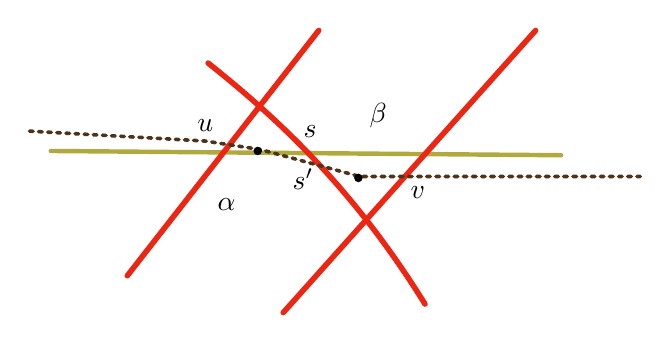
\begin{tikzpicture}[x=.018cm,y=-.018cm,line cap=round]
\draw[yellow!65!black,line width=1.6pt](365,1590)--(725,1593);
\draw[red!70!brown,line width=2pt](419,1678)--(554,1505) (476,1528)..controls(534,1574)and(583,1624)..(629,1698) (529,1704)--(707,1505);
\draw[brown!40!black,line width=1.3pt,dotted](350,1576)--(474,1583)--(513,1589)--(583,1608)--(781,1608);
\fill (511,1590) circle(3);\fill(582,1609)circle(3);
\node at(474,1572){$u$};\node at(489,1628){$\alpha$};\node at(596,1565){$\beta$};
\node at(548,1576){$s$};\node at(543,1610){$s'$};\node at(624,1619){$v$};
\end{tikzpicture}}
$\unsure{\overrightarrow{uv}|\widehat{uv}}$ (pointillé) sur
$\widetilde D_x$ est un arc
d'inertie (position
relative \uline{stable} donc). La circonstance
\unsure{propre} dans le cas où $(X,X_1)$ est un syst.
de ps. droites, et qui permet le contrôle
de ces sommets sur $\mathcal X$, est la suivante

\deleted{(PS) Soit $D$ une p.r. \deleted{\unsure{Étant} \unsure{le long duquel}
\uline{de ps dr} soit $s\in D\cap X_1$, et considérons
\unsure{le côté qui} \unsure{le} \unsure{$s',s''$} \inserted{antipolaires} \unsure{à} $s$ sur $D$, et un des arcs
déterminés \deleted{par} par $s',s''$ (appelons un
tel arc un \uline{demi-cercle} du polygone
top. ou comb. envisagé $\operatorname{Pol}(D)$), alors
\deleted{\unsure{on est sûr d'un demi-cercle}}\deleted{\unsure{sur $D$}}
\uline{si} sur $a$ il n'y a pas d'arc de
transition (``ordinaire'') alors $s\in X_0=S(X_1)$
etc.}
Soit $a$ un arc de transition \inserted{(ordinaire)}
sur $\widetilde D$, $a'$ l'arc opposé (donc $\bar a\cap\bar a'=\varnothing$)
et considérons \deleted{les} une des \inserted{$b$} comp. conn.
de $\widetilde D\setminus\{a\cup a'\}$. Alors, ou bien
$b$ contient un arc de transition \inserted{(ordinaire)}, ou
bien $b$ \deleted{\unsure{est une partie}} \inserted{est} un ``arc de
transition exceptionnel'', i.e. on est dans
l'un des cas suivants : on a une
``composante'' $D_i$ de $X_1$ qui est un cercle,
une \deleted{\unsure{sommet}} \inserted{facette $\varphi$ intermédiaire} (resp. une arête $\alpha$) sur $D_i$,
une orientation $\omega$ de $X$ en \deleted{\unsure{$\varphi$, une arête $a$ de}},
et $D$ est déduit de $(\deleted{\unsure{D_i}}\varphi,\omega)$ par
déformation élémentaire ---}
\figure{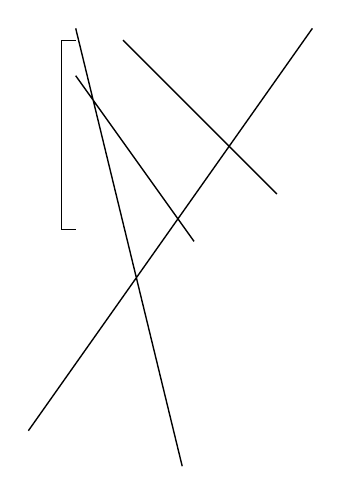
\begin{tikzpicture}[x=.003cm,y=.003cm]
\draw[line width=.5pt](0,0)--(450,-1850) (1000,0)--(-200,-1700) (200,-50)--(850,-700) (0,-200)--(500,-900);
\draw (0,-50)--(-60,-50)--(-60,-850)--(0,-850);
\end{tikzpicture}}
\margin{91}
